\documentclass{article} % For LaTeX2e
\usepackage{iclr2022_conference,times}
% Optional math commands from https://github.com/goodfeli/dlbook_notation.
%%%%% NEW MATH DEFINITIONS %%%%%

\usepackage{amsmath,amsfonts,bm}

% Mark sections of captions for referring to divisions of figures
\newcommand{\figleft}{{\em (Left)}}
\newcommand{\figcenter}{{\em (Center)}}
\newcommand{\figright}{{\em (Right)}}
\newcommand{\figtop}{{\em (Top)}}
\newcommand{\figbottom}{{\em (Bottom)}}
\newcommand{\captiona}{{\em (a)}}
\newcommand{\captionb}{{\em (b)}}
\newcommand{\captionc}{{\em (c)}}
\newcommand{\captiond}{{\em (d)}}

% Highlight a newly defined term
\newcommand{\newterm}[1]{{\bf #1}}


% Figure reference, lower-case.
\def\figref#1{figure~\ref{#1}}
% Figure reference, capital. For start of sentence
\def\Figref#1{Figure~\ref{#1}}
\def\twofigref#1#2{figures \ref{#1} and \ref{#2}}
\def\quadfigref#1#2#3#4{figures \ref{#1}, \ref{#2}, \ref{#3} and \ref{#4}}
% Section reference, lower-case.
\def\secref#1{section~\ref{#1}}
% Section reference, capital.
\def\Secref#1{Section~\ref{#1}}
% Reference to two sections.
\def\twosecrefs#1#2{sections \ref{#1} and \ref{#2}}
% Reference to three sections.
\def\secrefs#1#2#3{sections \ref{#1}, \ref{#2} and \ref{#3}}
% Reference to an equation, lower-case.
\def\eqref#1{equation~\ref{#1}}
% Reference to an equation, upper case
\def\Eqref#1{Equation~\ref{#1}}
% A raw reference to an equation---avoid using if possible
\def\plaineqref#1{\ref{#1}}
% Reference to a chapter, lower-case.
\def\chapref#1{chapter~\ref{#1}}
% Reference to an equation, upper case.
\def\Chapref#1{Chapter~\ref{#1}}
% Reference to a range of chapters
\def\rangechapref#1#2{chapters\ref{#1}--\ref{#2}}
% Reference to an algorithm, lower-case.
\def\algref#1{algorithm~\ref{#1}}
% Reference to an algorithm, upper case.
\def\Algref#1{Algorithm~\ref{#1}}
\def\twoalgref#1#2{algorithms \ref{#1} and \ref{#2}}
\def\Twoalgref#1#2{Algorithms \ref{#1} and \ref{#2}}
% Reference to a part, lower case
\def\partref#1{part~\ref{#1}}
% Reference to a part, upper case
\def\Partref#1{Part~\ref{#1}}
\def\twopartref#1#2{parts \ref{#1} and \ref{#2}}

\def\ceil#1{\lceil #1 \rceil}
\def\floor#1{\lfloor #1 \rfloor}
\def\1{\bm{1}}
\newcommand{\train}{\mathcal{D}}
\newcommand{\valid}{\mathcal{D_{\mathrm{valid}}}}
\newcommand{\test}{\mathcal{D_{\mathrm{test}}}}

\def\eps{{\epsilon}}


% Random variables
\def\reta{{\textnormal{$\eta$}}}
\def\ra{{\textnormal{a}}}
\def\rb{{\textnormal{b}}}
\def\rc{{\textnormal{c}}}
\def\rd{{\textnormal{d}}}
\def\re{{\textnormal{e}}}
\def\rf{{\textnormal{f}}}
\def\rg{{\textnormal{g}}}
\def\rh{{\textnormal{h}}}
\def\ri{{\textnormal{i}}}
\def\rj{{\textnormal{j}}}
\def\rk{{\textnormal{k}}}
\def\rl{{\textnormal{l}}}
% rm is already a command, just don't name any random variables m
\def\rn{{\textnormal{n}}}
\def\ro{{\textnormal{o}}}
\def\rp{{\textnormal{p}}}
\def\rq{{\textnormal{q}}}
\def\rr{{\textnormal{r}}}
\def\rs{{\textnormal{s}}}
\def\rt{{\textnormal{t}}}
\def\ru{{\textnormal{u}}}
\def\rv{{\textnormal{v}}}
\def\rw{{\textnormal{w}}}
\def\rx{{\textnormal{x}}}
\def\ry{{\textnormal{y}}}
\def\rz{{\textnormal{z}}}

% Random vectors
\def\rvepsilon{{\mathbf{\epsilon}}}
\def\rvtheta{{\mathbf{\theta}}}
\def\rva{{\mathbf{a}}}
\def\rvb{{\mathbf{b}}}
\def\rvc{{\mathbf{c}}}
\def\rvd{{\mathbf{d}}}
\def\rve{{\mathbf{e}}}
\def\rvf{{\mathbf{f}}}
\def\rvg{{\mathbf{g}}}
\def\rvh{{\mathbf{h}}}
\def\rvu{{\mathbf{i}}}
\def\rvj{{\mathbf{j}}}
\def\rvk{{\mathbf{k}}}
\def\rvl{{\mathbf{l}}}
\def\rvm{{\mathbf{m}}}
\def\rvn{{\mathbf{n}}}
\def\rvo{{\mathbf{o}}}
\def\rvp{{\mathbf{p}}}
\def\rvq{{\mathbf{q}}}
\def\rvr{{\mathbf{r}}}
\def\rvs{{\mathbf{s}}}
\def\rvt{{\mathbf{t}}}
\def\rvu{{\mathbf{u}}}
\def\rvv{{\mathbf{v}}}
\def\rvw{{\mathbf{w}}}
\def\rvx{{\mathbf{x}}}
\def\rvy{{\mathbf{y}}}
\def\rvz{{\mathbf{z}}}

% Elements of random vectors
\def\erva{{\textnormal{a}}}
\def\ervb{{\textnormal{b}}}
\def\ervc{{\textnormal{c}}}
\def\ervd{{\textnormal{d}}}
\def\erve{{\textnormal{e}}}
\def\ervf{{\textnormal{f}}}
\def\ervg{{\textnormal{g}}}
\def\ervh{{\textnormal{h}}}
\def\ervi{{\textnormal{i}}}
\def\ervj{{\textnormal{j}}}
\def\ervk{{\textnormal{k}}}
\def\ervl{{\textnormal{l}}}
\def\ervm{{\textnormal{m}}}
\def\ervn{{\textnormal{n}}}
\def\ervo{{\textnormal{o}}}
\def\ervp{{\textnormal{p}}}
\def\ervq{{\textnormal{q}}}
\def\ervr{{\textnormal{r}}}
\def\ervs{{\textnormal{s}}}
\def\ervt{{\textnormal{t}}}
\def\ervu{{\textnormal{u}}}
\def\ervv{{\textnormal{v}}}
\def\ervw{{\textnormal{w}}}
\def\ervx{{\textnormal{x}}}
\def\ervy{{\textnormal{y}}}
\def\ervz{{\textnormal{z}}}

% Random matrices
\def\rmA{{\mathbf{A}}}
\def\rmB{{\mathbf{B}}}
\def\rmC{{\mathbf{C}}}
\def\rmD{{\mathbf{D}}}
\def\rmE{{\mathbf{E}}}
\def\rmF{{\mathbf{F}}}
\def\rmG{{\mathbf{G}}}
\def\rmH{{\mathbf{H}}}
\def\rmI{{\mathbf{I}}}
\def\rmJ{{\mathbf{J}}}
\def\rmK{{\mathbf{K}}}
\def\rmL{{\mathbf{L}}}
\def\rmM{{\mathbf{M}}}
\def\rmN{{\mathbf{N}}}
\def\rmO{{\mathbf{O}}}
\def\rmP{{\mathbf{P}}}
\def\rmQ{{\mathbf{Q}}}
\def\rmR{{\mathbf{R}}}
\def\rmS{{\mathbf{S}}}
\def\rmT{{\mathbf{T}}}
\def\rmU{{\mathbf{U}}}
\def\rmV{{\mathbf{V}}}
\def\rmW{{\mathbf{W}}}
\def\rmX{{\mathbf{X}}}
\def\rmY{{\mathbf{Y}}}
\def\rmZ{{\mathbf{Z}}}

% Elements of random matrices
\def\ermA{{\textnormal{A}}}
\def\ermB{{\textnormal{B}}}
\def\ermC{{\textnormal{C}}}
\def\ermD{{\textnormal{D}}}
\def\ermE{{\textnormal{E}}}
\def\ermF{{\textnormal{F}}}
\def\ermG{{\textnormal{G}}}
\def\ermH{{\textnormal{H}}}
\def\ermI{{\textnormal{I}}}
\def\ermJ{{\textnormal{J}}}
\def\ermK{{\textnormal{K}}}
\def\ermL{{\textnormal{L}}}
\def\ermM{{\textnormal{M}}}
\def\ermN{{\textnormal{N}}}
\def\ermO{{\textnormal{O}}}
\def\ermP{{\textnormal{P}}}
\def\ermQ{{\textnormal{Q}}}
\def\ermR{{\textnormal{R}}}
\def\ermS{{\textnormal{S}}}
\def\ermT{{\textnormal{T}}}
\def\ermU{{\textnormal{U}}}
\def\ermV{{\textnormal{V}}}
\def\ermW{{\textnormal{W}}}
\def\ermX{{\textnormal{X}}}
\def\ermY{{\textnormal{Y}}}
\def\ermZ{{\textnormal{Z}}}

% Vectors
\def\vzero{{\bm{0}}}
\def\vone{{\bm{1}}}
\def\vmu{{\bm{\mu}}}
\def\vtheta{{\bm{\theta}}}
\def\va{{\bm{a}}}
\def\vb{{\bm{b}}}
\def\vc{{\bm{c}}}
\def\vd{{\bm{d}}}
\def\ve{{\bm{e}}}
\def\vf{{\bm{f}}}
\def\vg{{\bm{g}}}
\def\vh{{\bm{h}}}
\def\vi{{\bm{i}}}
\def\vj{{\bm{j}}}
\def\vk{{\bm{k}}}
\def\vl{{\bm{l}}}
\def\vm{{\bm{m}}}
\def\vn{{\bm{n}}}
\def\vo{{\bm{o}}}
\def\vp{{\bm{p}}}
\def\vq{{\bm{q}}}
\def\vr{{\bm{r}}}
\def\vs{{\bm{s}}}
\def\vt{{\bm{t}}}
\def\vu{{\bm{u}}}
\def\vv{{\bm{v}}}
\def\vw{{\bm{w}}}
\def\vx{{\bm{x}}}
\def\vy{{\bm{y}}}
\def\vz{{\bm{z}}}

% Elements of vectors
\def\evalpha{{\alpha}}
\def\evbeta{{\beta}}
\def\evepsilon{{\epsilon}}
\def\evlambda{{\lambda}}
\def\evomega{{\omega}}
\def\evmu{{\mu}}
\def\evpsi{{\psi}}
\def\evsigma{{\sigma}}
\def\evtheta{{\theta}}
\def\eva{{a}}
\def\evb{{b}}
\def\evc{{c}}
\def\evd{{d}}
\def\eve{{e}}
\def\evf{{f}}
\def\evg{{g}}
\def\evh{{h}}
\def\evi{{i}}
\def\evj{{j}}
\def\evk{{k}}
\def\evl{{l}}
\def\evm{{m}}
\def\evn{{n}}
\def\evo{{o}}
\def\evp{{p}}
\def\evq{{q}}
\def\evr{{r}}
\def\evs{{s}}
\def\evt{{t}}
\def\evu{{u}}
\def\evv{{v}}
\def\evw{{w}}
\def\evx{{x}}
\def\evy{{y}}
\def\evz{{z}}

% Matrix
\def\mA{{\bm{A}}}
\def\mB{{\bm{B}}}
\def\mC{{\bm{C}}}
\def\mD{{\bm{D}}}
\def\mE{{\bm{E}}}
\def\mF{{\bm{F}}}
\def\mG{{\bm{G}}}
\def\mH{{\bm{H}}}
\def\mI{{\bm{I}}}
\def\mJ{{\bm{J}}}
\def\mK{{\bm{K}}}
\def\mL{{\bm{L}}}
\def\mM{{\bm{M}}}
\def\mN{{\bm{N}}}
\def\mO{{\bm{O}}}
\def\mP{{\bm{P}}}
\def\mQ{{\bm{Q}}}
\def\mR{{\bm{R}}}
\def\mS{{\bm{S}}}
\def\mT{{\bm{T}}}
\def\mU{{\bm{U}}}
\def\mV{{\bm{V}}}
\def\mW{{\bm{W}}}
\def\mX{{\bm{X}}}
\def\mY{{\bm{Y}}}
\def\mZ{{\bm{Z}}}
\def\mBeta{{\bm{\beta}}}
\def\mPhi{{\bm{\Phi}}}
\def\mLambda{{\bm{\Lambda}}}
\def\mSigma{{\bm{\Sigma}}}

% Tensor
\DeclareMathAlphabet{\mathsfit}{\encodingdefault}{\sfdefault}{m}{sl}
\SetMathAlphabet{\mathsfit}{bold}{\encodingdefault}{\sfdefault}{bx}{n}
\newcommand{\tens}[1]{\bm{\mathsfit{#1}}}
\def\tA{{\tens{A}}}
\def\tB{{\tens{B}}}
\def\tC{{\tens{C}}}
\def\tD{{\tens{D}}}
\def\tE{{\tens{E}}}
\def\tF{{\tens{F}}}
\def\tG{{\tens{G}}}
\def\tH{{\tens{H}}}
\def\tI{{\tens{I}}}
\def\tJ{{\tens{J}}}
\def\tK{{\tens{K}}}
\def\tL{{\tens{L}}}
\def\tM{{\tens{M}}}
\def\tN{{\tens{N}}}
\def\tO{{\tens{O}}}
\def\tP{{\tens{P}}}
\def\tQ{{\tens{Q}}}
\def\tR{{\tens{R}}}
\def\tS{{\tens{S}}}
\def\tT{{\tens{T}}}
\def\tU{{\tens{U}}}
\def\tV{{\tens{V}}}
\def\tW{{\tens{W}}}
\def\tX{{\tens{X}}}
\def\tY{{\tens{Y}}}
\def\tZ{{\tens{Z}}}


% Graph
\def\gA{{\mathcal{A}}}
\def\gB{{\mathcal{B}}}
\def\gC{{\mathcal{C}}}
\def\gD{{\mathcal{D}}}
\def\gE{{\mathcal{E}}}
\def\gF{{\mathcal{F}}}
\def\gG{{\mathcal{G}}}
\def\gH{{\mathcal{H}}}
\def\gI{{\mathcal{I}}}
\def\gJ{{\mathcal{J}}}
\def\gK{{\mathcal{K}}}
\def\gL{{\mathcal{L}}}
\def\gM{{\mathcal{M}}}
\def\gN{{\mathcal{N}}}
\def\gO{{\mathcal{O}}}
\def\gP{{\mathcal{P}}}
\def\gQ{{\mathcal{Q}}}
\def\gR{{\mathcal{R}}}
\def\gS{{\mathcal{S}}}
\def\gT{{\mathcal{T}}}
\def\gU{{\mathcal{U}}}
\def\gV{{\mathcal{V}}}
\def\gW{{\mathcal{W}}}
\def\gX{{\mathcal{X}}}
\def\gY{{\mathcal{Y}}}
\def\gZ{{\mathcal{Z}}}

% Sets
\def\sA{{\mathbb{A}}}
\def\sB{{\mathbb{B}}}
\def\sC{{\mathbb{C}}}
\def\sD{{\mathbb{D}}}
% Don't use a set called E, because this would be the same as our symbol
% for expectation.
\def\sF{{\mathbb{F}}}
\def\sG{{\mathbb{G}}}
\def\sH{{\mathbb{H}}}
\def\sI{{\mathbb{I}}}
\def\sJ{{\mathbb{J}}}
\def\sK{{\mathbb{K}}}
\def\sL{{\mathbb{L}}}
\def\sM{{\mathbb{M}}}
\def\sN{{\mathbb{N}}}
\def\sO{{\mathbb{O}}}
\def\sP{{\mathbb{P}}}
\def\sQ{{\mathbb{Q}}}
\def\sR{{\mathbb{R}}}
\def\sS{{\mathbb{S}}}
\def\sT{{\mathbb{T}}}
\def\sU{{\mathbb{U}}}
\def\sV{{\mathbb{V}}}
\def\sW{{\mathbb{W}}}
\def\sX{{\mathbb{X}}}
\def\sY{{\mathbb{Y}}}
\def\sZ{{\mathbb{Z}}}

% Entries of a matrix
\def\emLambda{{\Lambda}}
\def\emA{{A}}
\def\emB{{B}}
\def\emC{{C}}
\def\emD{{D}}
\def\emE{{E}}
\def\emF{{F}}
\def\emG{{G}}
\def\emH{{H}}
\def\emI{{I}}
\def\emJ{{J}}
\def\emK{{K}}
\def\emL{{L}}
\def\emM{{M}}
\def\emN{{N}}
\def\emO{{O}}
\def\emP{{P}}
\def\emQ{{Q}}
\def\emR{{R}}
\def\emS{{S}}
\def\emT{{T}}
\def\emU{{U}}
\def\emV{{V}}
\def\emW{{W}}
\def\emX{{X}}
\def\emY{{Y}}
\def\emZ{{Z}}
\def\emSigma{{\Sigma}}

% entries of a tensor
% Same font as tensor, without \bm wrapper
\newcommand{\etens}[1]{\mathsfit{#1}}
\def\etLambda{{\etens{\Lambda}}}
\def\etA{{\etens{A}}}
\def\etB{{\etens{B}}}
\def\etC{{\etens{C}}}
\def\etD{{\etens{D}}}
\def\etE{{\etens{E}}}
\def\etF{{\etens{F}}}
\def\etG{{\etens{G}}}
\def\etH{{\etens{H}}}
\def\etI{{\etens{I}}}
\def\etJ{{\etens{J}}}
\def\etK{{\etens{K}}}
\def\etL{{\etens{L}}}
\def\etM{{\etens{M}}}
\def\etN{{\etens{N}}}
\def\etO{{\etens{O}}}
\def\etP{{\etens{P}}}
\def\etQ{{\etens{Q}}}
\def\etR{{\etens{R}}}
\def\etS{{\etens{S}}}
\def\etT{{\etens{T}}}
\def\etU{{\etens{U}}}
\def\etV{{\etens{V}}}
\def\etW{{\etens{W}}}
\def\etX{{\etens{X}}}
\def\etY{{\etens{Y}}}
\def\etZ{{\etens{Z}}}

% The true underlying data generating distribution
\newcommand{\pdata}{p_{\rm{data}}}
% The empirical distribution defined by the training set
\newcommand{\ptrain}{\hat{p}_{\rm{data}}}
\newcommand{\Ptrain}{\hat{P}_{\rm{data}}}
% The model distribution
\newcommand{\pmodel}{p_{\rm{model}}}
\newcommand{\Pmodel}{P_{\rm{model}}}
\newcommand{\ptildemodel}{\tilde{p}_{\rm{model}}}
% Stochastic autoencoder distributions
\newcommand{\pencode}{p_{\rm{encoder}}}
\newcommand{\pdecode}{p_{\rm{decoder}}}
\newcommand{\precons}{p_{\rm{reconstruct}}}

\newcommand{\laplace}{\mathrm{Laplace}} % Laplace distribution

\newcommand{\E}{\mathbb{E}}
\newcommand{\Ls}{\mathcal{L}}
\newcommand{\R}{\mathbb{R}}
\newcommand{\emp}{\tilde{p}}
\newcommand{\lr}{\alpha}
\newcommand{\reg}{\lambda}
\newcommand{\rect}{\mathrm{rectifier}}
\newcommand{\softmax}{\mathrm{softmax}}
\newcommand{\sigmoid}{\sigma}
\newcommand{\softplus}{\zeta}
\newcommand{\KL}{D_{\mathrm{KL}}}
\newcommand{\Var}{\mathrm{Var}}
\newcommand{\standarderror}{\mathrm{SE}}
\newcommand{\Cov}{\mathrm{Cov}}
% Wolfram Mathworld says $L^2$ is for function spaces and $\ell^2$ is for vectors
% But then they seem to use $L^2$ for vectors throughout the site, and so does
% wikipedia.
\newcommand{\normlzero}{L^0}
\newcommand{\normlone}{L^1}
\newcommand{\normltwo}{L^2}
\newcommand{\normlp}{L^p}
\newcommand{\normmax}{L^\infty}

\newcommand{\parents}{Pa} % See usage in notation.tex. Chosen to match Daphne's book.

\DeclareMathOperator*{\argmax}{arg\,max}
\DeclareMathOperator*{\argmin}{arg\,min}

\DeclareMathOperator{\sign}{sign}
\DeclareMathOperator{\Tr}{Tr}
\let\ab\allowbreak


%######## APS360: Uncomment your submission name
%\newcommand{\apsname}{Project Proposal}
\newcommand{\apsname}{Progress Report}
%\newcommand{\apsname}{Final Report}

%######## APS360: Put your Group Number here
\newcommand{\gpnumber}{40}

\usepackage{hyperref}
\usepackage{xcolor}
\usepackage[normalem]{ulem}
\usepackage{url}
\usepackage{graphicx}

%######## APS360: Put your project Title here
\title{Image Colourization via Convolutional \\
Neural Networks and Deep Learning}

%######## APS360: Put your names, student IDs and Emails here
\author{Youssef Fikry  \\
Student\# 1005678901\\
\texttt{youssef.fikry@mail.utoronto.ca} \\
\And Harkirpa Kaur  \\
Student\# 1011242479 \\
\texttt{harkirpa.kaur@mail.utoronto.ca} \\
\AND
Peter Leong \\
Student\# 1005678901 \\
\texttt{peter.leong@mail.utoronto.ca} \\
\And
Thulasi Thavarajah \\
Student\# 10115358424 \\
\texttt{t.thavarajah@mail.utoronto.ca} \\
\AND
}

% The \author macro works with any number of authors. There are two commands
% used to separate the names and addresses of multiple authors: \And and \AND.
%
% Using \And between authors leaves it to \LaTeX{} to determine where to break
% the lines. Using \AND forces a linebreak at that point. So, if \LaTeX{}
% puts 3 of 4 authors names on the first line, and the last on the second
% line, try using \AND instead of \And before the third author name.

\newcommand{\fix}{\marginpar{FIX}}
\newcommand{\new}{\marginpar{NEW}}

\iclrfinalcopy 
%######## APS360: Document starts here
\begin{document}


\maketitle

\begin{abstract}
This project addresses the challenge of automated colourization for 256$\times$256 grayscale images using a dataset of 12,600 image pairs, balanced across human subjects, 
animals, and natural scenery. We frame colourization as a supervised learning problem in the CIELAB colour space, where a model predicts chrominance channels ($a^*$, $b^*$) 
from the luminance channel ($L^*$). A shallow convolutional neural network (CNN) provides the baseline performance, while our primary solution employs a deeper convolutional encoder-decoder architecture. This 
design captures high-level semantic features and spatial context, addressing limitations of shallow networks in perceptual realism. All source code, datasets, and results 
are publicly available \href{https://drive.google.com/drive/folders/1cV1NhlQ8UTk_CgJdwhqeRu0z5xE85ZsI?usp=sharing}{here}. 
%######## APS360: Do not change the next line. This shows your Main body page count.
----Total Pages: \pageref{last_page}
\end{abstract}


\section{Brief Project Description}

The invention of photography provided the technology to capture a moment in time. However, for most of photographic history, the process of obtaining coloured images eluded photographers \citep{scienceandmediamuseum2020}. As a result, much of historic photography is grayscale; lacking the visual richness found in modern photography and is inaccessible to individuals with vision impairments \citep{vogelsang2024impact}. This project aims to leverage deep learning to automate the colorization of grayscale images, thereby aiding in the revitalization of grayscale photographs. Furthermore, image colorization technology assists archivists and museums in restoring lost visual information and has applications in the media, medical and geospatial industries. 

Traditional image colorization methods involve manual labour that is costly and time-consuming \citep{farella2022}. On the other hand, deep learning approaches automate the colorization process and supplant traditional techniques \citep{farella2022}. In machine learning, colorization is defined as a model taking a black-and-white image as an input, and outputting its coloured counterpart \citep{lettherebecolor}. From a machine learning perspective, deep convolutional neural networks are best suited for this task as they can extract and learn features such as colors, patterns and shapes in images and affiliate them with object classes \citep{deepcnn}. These characteristics aid CNNs in excelling at object classificition tasks, as well as image colorization \citep{deepcnn}. 

//insert image here. 

\section{Individual Contributions \& Responsibilities}

\section{Notable Contribution}

\subsection{Data Processing}

 The team compiled the project's image dataset using Kaggle.com, an online platform that provides access to publicly available, real-world datasets and a community for data scientists \citep[]{kaggle}. The final dataset for this project has three classes: human, animal, and scenic.  To train a model that can generalize to a broad range of images, the final dataset for this project includes three categories:. All selected datasets are licensed for public domain use. 

 \subsubsection{Repurposing Online Datasets}

The human image dataset, originally intended for human detection, contains a diverse range of 17,300 images of people in different environments \citep[]{kaggle_human}. Furthermore, the animal image dataset, initially developed for image classification contains 5,400 images of 90 different animals \citep[]{kaggle_animal}. For this project’s purpose, this dataset is ideal as it encompasses a diverse set of images with an equal distribution of each animal. Additionally, the scenic image dataset from \citet{kaggle_scene} contains 4,319 images of a variety of landscapes spanning a large breadth of colour palettes, potentially influencing the robustness of the final model.

\subsubsection{Cleaning Up The Datasets}
The team extracted all the images from each dataset and relocated them into folders corresponding to their category (human/animal/scenic). Due to the disparity in the size of the three datasets, each dataset was reduced to exactly 4200 images using Python’s \verb|random.sample| function with the seed set to 42. The images were then renamed in accordance to their respective categories (ex. human\_0001.jpg). 

\subsubsection{Formatting the Data}

This project requires a unique dataset with black-and-white images paired with their coloured counterparts as the ground truths. To format the cleaned up data and create this dataset, PyTorch’s \verb|torchvision.transforms| library was utiltized. The team first converted the original images into 256 x 256 pixel ground truth images using the \verb|Resize| transform and sorted them according to their category. Following this, \verb|Grayscale| transform with a output channel of 1 was used to convert the 256 x 256 pixel colour images to 256 x 256 pixel grayscale images to feed into the model. 

 \subsubsection{Splitting Dataset Into Training, Validation and Test Sets}

To create the training, validation and test sets, a ratio of 70:15:15 was chosen. The first 2940 images of each of dataset categories (human/animal/scene) were selected for the training set. The remaining images were split evenly to create the validation and testing datasets. 

\subsubsection{The Final Dataset}

The final dataset is composed of 12,600 pairs of colour and their corresponding grayscale images. Each category (human, animal, and scenic) contains 4,200 image pairs and an even distribution of each category was maintained in the training, validation and test sets.

\begin{figure}[htbp]            % h=here, t=top, b=bottom, p=page float
  \centering
  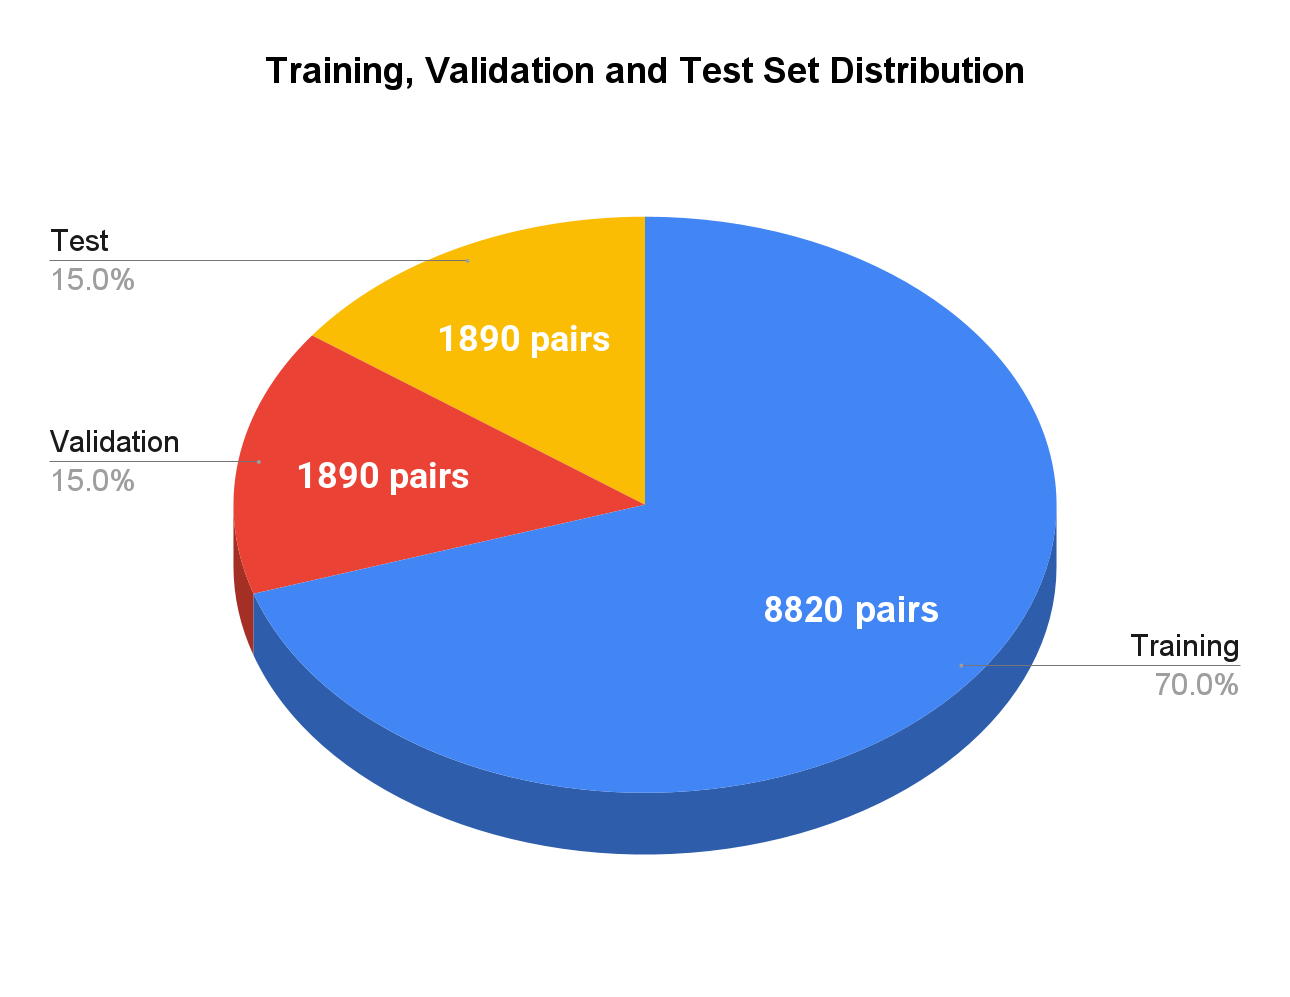
\includegraphics[width=0.65\linewidth]{Figs/dataset1.png}
  \caption{Training, Validation and Test Set Distribution of 12600 Image Pairs}
  \label{fig:dataset}
\end{figure}

\begin{figure}[htbp]            % h=here, t=top, b=bottom, p=page float
  \centering
  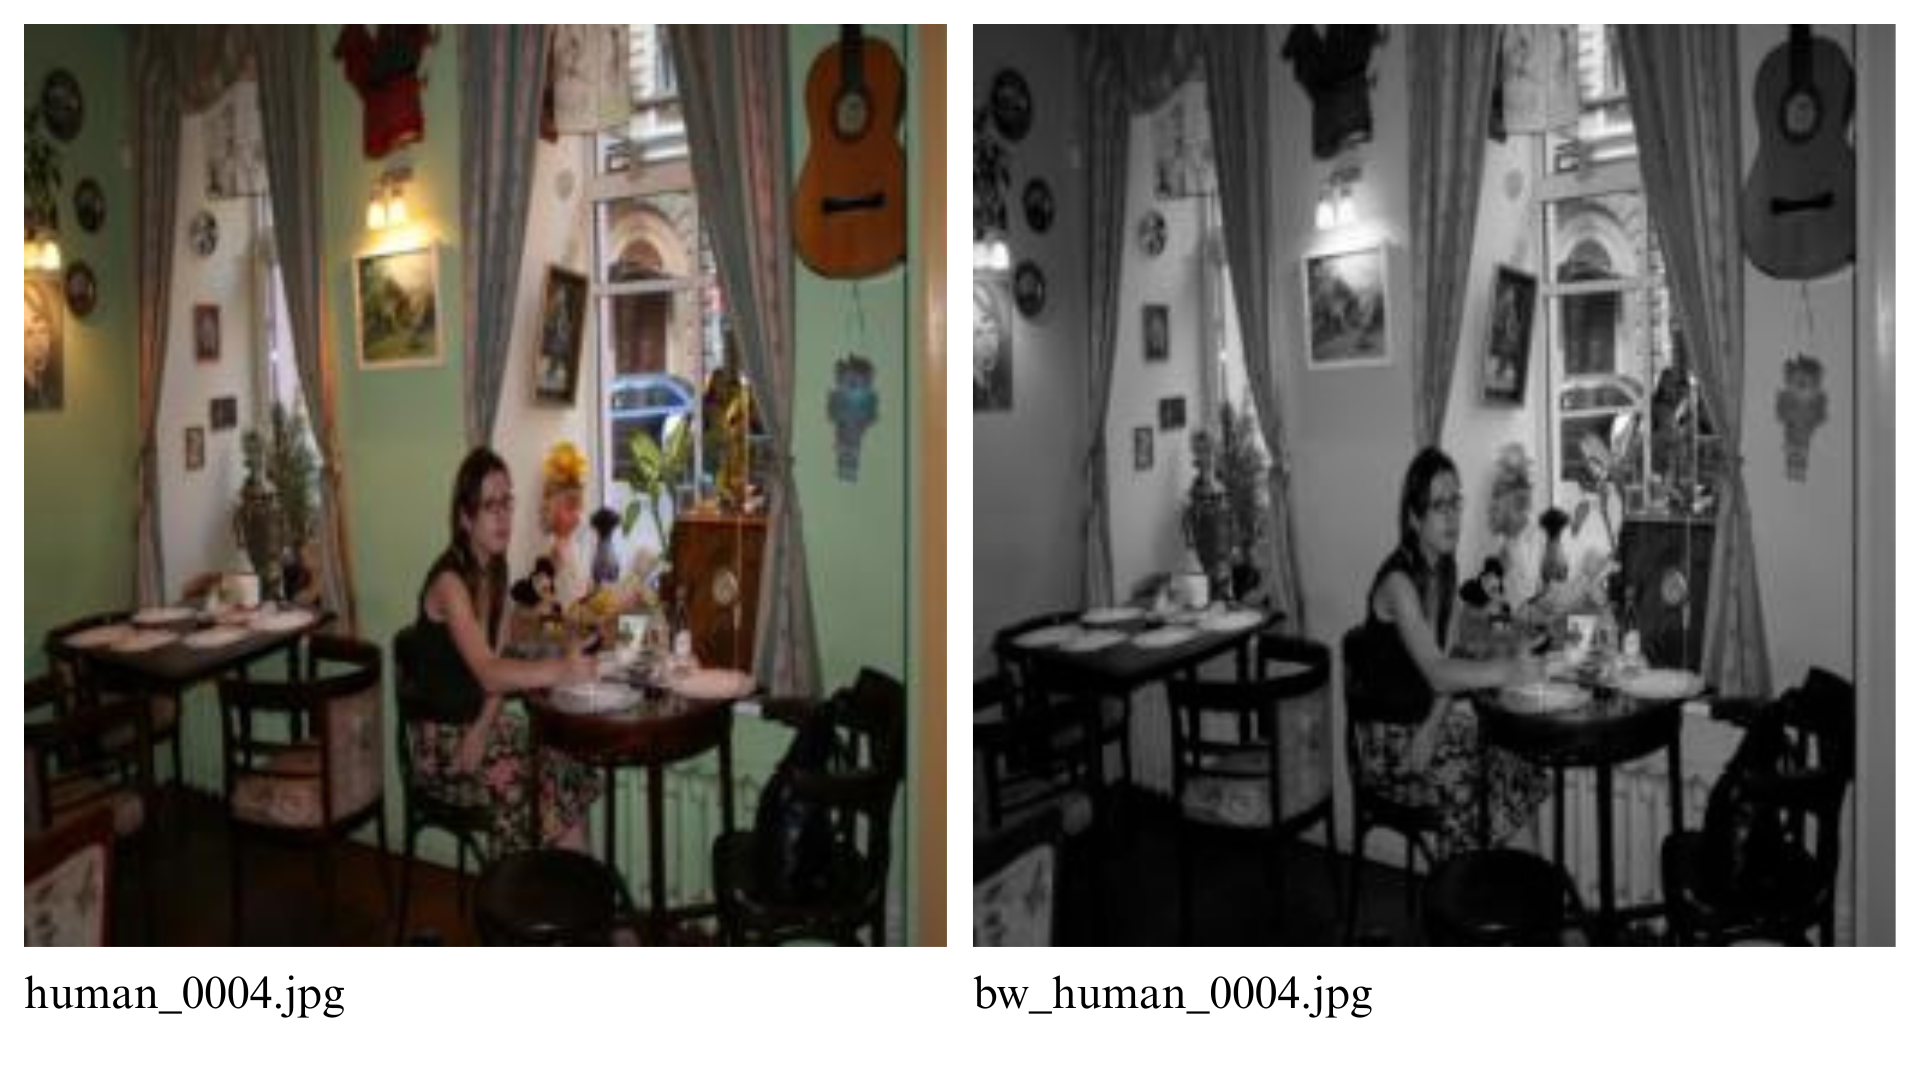
\includegraphics[width=0.65\linewidth]{Figs/Data Example.png}
  \caption{Sample Data Pair from Training Set}
  \label{fig:data_example}
\end{figure}b

\subsection{Baseline Model}

To establish a performance benchmark for our colorization task, we implemented a shallow convolutional neural network called \texttt{ShallowColorizationNet}. This model uses a simple 
encoder-bottleneck-decoder architecture and does not incorporate adversarial training. Its purpose is to test the feasibility of learning a direct mapping from grayscale luminance (\textit{L}) 
input to the chrominance (\textit{ab}) channels in the CIELAB color space.

\subsubsection{Model Architecture}

The architecture of the baseline model is as follows:
\begin{itemize}
    \item \textbf{Encoder:} Two convolutional layers with ReLU activation followed by max pooling, reducing spatial dimensions while increasing channel depth.
    \item \textbf{Bottleneck:} A single convolutional layer that expands the feature representation.
    \item \textbf{Decoder:} A transposed convolution to restore spatial resolution and a final convolutional layer outputting two channels (for \textit{a} and \textit{b}), with a $\tanh$ 
    activation to constrain values between $[-1, 1]$.
\end{itemize}

\subsubsection{Training and Comparison Approach}

The baseline model was trained using the L1 loss between predicted and ground truth \textit{ab} channels. This model was compared to our primary neural network—a conditional 
GAN model that includes a discriminator to encourage more realistic colorizations—based on both quantitative and qualitative results.

\subsubsection{Quantitative and Qualitative Results}

\textbf{Quantitative:} The baseline model was trained for 5 epochs using L1 loss. The generator's loss remained stable around \textbf{1.5647}, while the discriminator's loss 
converged to approximately \textbf{0.7074}. These consistent values suggest that the baseline network was able to learn a basic mapping from grayscale to chrominance, but likely 
lacked the capacity or incentive to produce high-fidelity or diverse outputs. These values serve as reference points for evaluating improvements made by our primary GAN-based model.

\begin{figure}[htbp]
    \centering
    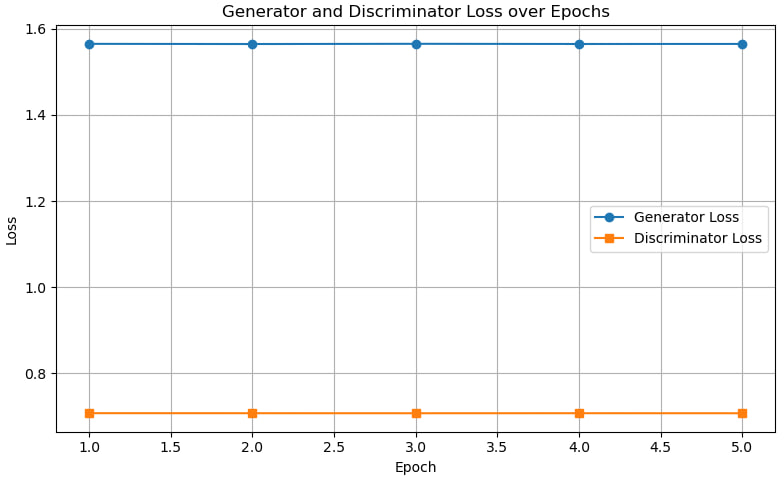
\includegraphics[width=\textwidth]{Figs/baseline_learning_curve.jpg}
    \caption{Generator and discriminator loss values over 5 epochs of training. The architecture will be investigated further during the final phase of the project to determine why 
    the loss values fluctuate by such small amounts.}

    \label{fig:baseline_outputs}
\end{figure}

\textbf{Qualitative:} The baseline model produced smooth but somewhat desaturated colorizations. It tended to predict average colors in ambiguous regions, resulting in low color 
diversity. See Figure~\ref{fig:baseline_outputs} for representative examples.

\begin{figure}[htbp]
    \centering
    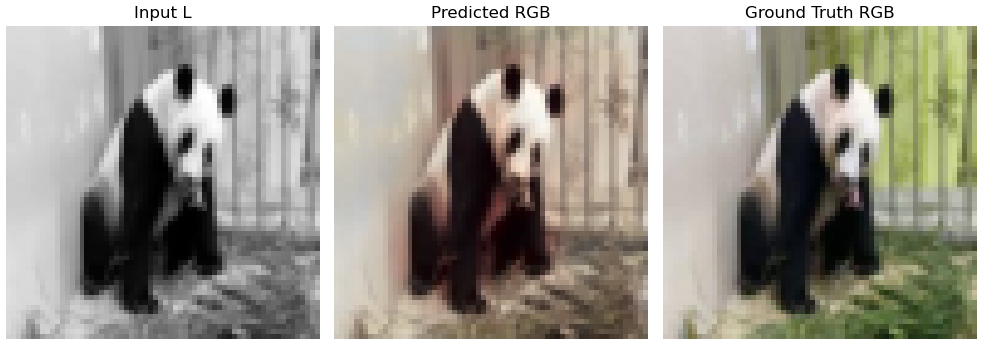
\includegraphics[width=\textwidth]{Figs/baseline_output.png}
    \caption{Sample output from the baseline model on grayscale input images.}
    \label{fig:baseline_outputs}
\end{figure}

\subsubsection{Challenges}

The primary challenge encountered during development was the tendency of the baseline model to learn overly conservative color predictions. Without a discriminator or explicit 
diversity loss, the network favored colorizations close to the dataset mean. Additionally, selecting the appropriate normalization strategy for LAB space and constraining output to 
valid chrominance ranges required careful tuning.

\subsubsection{Feasibility Assessment}

Despite its simplicity, the baseline model demonstrated that the colorization task is learnable with a low-capacity network, although the outputs lacked the vividness and fidelity 
achieved by our primary GAN-based model. The baseline thus served its role in confirming the viability of end-to-end colorization from grayscale input and establishing a benchmark 
for model improvement.

\subsection{Primary Model}

Our colouriser combines a lightweight ResNet-18 encoder with a U-Net decoder. This design keeps global scene context (from the pretrained encoder) while preserving fine edges through skip connections, all within a 15 M-parameter budget suitable for Google Colab.

\subsubsection{Architecture}

The encoder copies the first four blocks of ResNet-18, pretrained on ImageNet, but the opening convolution is modified to ingest a single-channel L image. Feature maps are therefore produced at 256×256, 128×128, 64×64 and 32×32.
A symmetric decoder upsamples in three steps (transpose-conv → 3 × 3 conv × 2, BatchNorm, ReLU). Skip links inject the corresponding encoder features to keep edges crisp. A final 3 × 3 layer with tanh activation outputs the a and b chroma channels. Total capacity is ~15 M parameters, comfortably below Colab’s memory ceiling. The whole network sits under 25 MB on disk, so checkpoints save quickly.

\subsubsection{Training Progress}

We train with AdamW (lr = 3 × $10^{-4}$, batch = 32) on the cleaned 12.6 k-image set, and the learning rate decays each epoch via cosine annealing. Five epochs on a pro A100 GPU took just under 20 minutes. Validation L1 dropped from 0.07 to 0.0064, and SSIM climbed from 0.58 to 0.74. Qualitatively the model recovers plausible sky blues and fur textures that the two-layer baseline could not capture. The model also learns to colorize human skin tones, but it struggles with complex scenes like forests and crowds, where it tends to produce muddy colors.

\subsubsection{Challenges}

On some photos the network over-uses warm hues, giving a slight brown cast. Early inspection shows that brown-dominant scenes are over-represented in the training set and the loss does not penalise colour bias. We plan to rebalance LAB histograms per batch and add a small perceptual term to discourage monotone outputs.

\subsubsection{Feasibility Assessment}

After five epochs the model already lifts SSIM from 0.58 (baseline) to 0.74, showing it can learn credible colour cues. Remaining errors are mostly a warm “brown” bias. Because these mistakes are consistent, modest adjustments should yield clear gains. We plan to (i) rebalance training batches so cool and warm tones appear equally, and (ii) add a light perceptual loss to discourage over-use of one hue. These changes require no extra parameters or memory. With a 20-epoch run and a cosine learning-rate schedule, we expect further improvement toward an SSIM of 0.80 while staying within course limits.

\label{last_page}

\newpage
\bibliographystyle{iclr2022_conference}
\bibliography{APS360_Report_ref}

\end{document}
